\documentclass[conference]{IEEEtran}
\usepackage{iftex}
\ifPDFTeX
  \usepackage[T1]{fontenc}
  \usepackage[utf8]{inputenc}
\else
  \usepackage{fontspec}
  \setmainfont{texgyretermes}[Extension=.otf,UprightFont=*-regular,
    BoldFont=*-bold,ItalicFont=*-italic,BoldItalicFont=*-bolditalic]
\fi
\usepackage{cite}
\usepackage{amsmath,amssymb}
\usepackage{graphicx}
\usepackage{booktabs}
\usepackage{xcolor}
\definecolor{modelLunaDecisions}{HTML}{234E70}
\definecolor{modelLunaChat}{HTML}{087F8C}
\definecolor{modelJev}{HTML}{7C3AED}
\definecolor{modelJev114}{HTML}{2563EB}
\definecolor{modelDecider}{HTML}{00856A}
\definecolor{modelClef}{HTML}{B45309}
\definecolor{modelClefFlash}{HTML}{BE185D}
\newcommand{\modelname}[2]{\textcolor{#1}{\textbullet}\,\textnormal{#2}}
\newcommand{\tablehead}[1]{\shortstack{#1}}
\usepackage{url}
\usepackage[hidelinks]{hyperref}
\graphicspath{{figures/}}
\newcommand{\yes}{\textsc{yes}}
\newcommand{\no}{\textsc{no}}
\newcommand{\NA}{\textsc{na}}
\hyphenation{Gold-fish-Bench}

\begin{document}
\title{GoldfishBench: Separating Intervention Need from the Suitability of a Named Recipient}
\author{\IEEEauthorblockN{Muhammed Izzet Sezer}
\IEEEauthorblockA{\texttt{i@imsezer.com}}}
\maketitle

\begin{abstract}
Decision models can approve or reject requests in organizational workflows.
GoldfishBench tests whether they distinguish two questions: does a task need
intervention, and can the proposed recipient actually perform it? Under our
explicit policy, routing is correct only when both conditions hold. We evaluate
six decision-model conditions, including two Jev versions, and one general-purpose
language-model classifier on 662 scenario families, yielding 55,603 usable routing
answers. We vary intervention need, recipient suitability and request wording.
For an unsuitable recipient, the correct answer is always NO. Yet OpenAI GPT-6
Luna Decisions approves 470 of 662 such requests when intervention is needed
under the name/prose condition, compared with 2 of 662 when it is not. Keeping
task and capabilities fixed, changing names and prose raises this model's
false-approval rate by 23.26 percentage points; urgency raises TypeSafe Jev
1.13's rate by 21.00 points. Effects differ across models: Perplexity Decider V1.2
correctly answers all 7,944 joint routing questions. Separate component questions
also reveal cases where correct component answers coexist with a wrong joint
answer. High overall scores can conceal frequent approval of unsuitable
recipients, while successful systems limit any universal persuasion claim.
These exploratory results concern synthetic scenarios without independent human
semantic validation, not demonstrated attacks on deployed services.
\end{abstract}

\begingroup
\renewcommand{\abstractname}{Özet}
\begin{abstract}
Karar modelleri, kurumsal iş akışlarında talepleri onaylamak veya reddetmek için
kullanılabilir. GoldfishBench iki sorunun birbirinden ayrılıp ayrılmadığını
inceler: İşe müdahale etmek gerekiyor mu ve önerilen kişi, ekip veya hizmet bu işi
yapabilir mi? Kuralımıza göre yönlendirme ancak iki koşul da sağlandığında
onaylanmalıdır. Jev'in iki sürümü dahil altı karar modeli koşulunu ve karşılaştırma
için bir genel amaçlı dil modelini, 662 senaryo ailesinde 55.603 kullanılabilir
yönlendirme yanıtıyla değerlendiriyoruz. Müdahale ihtiyacını, alıcının uygunluğunu
ve talebin ifade edilişini değiştiriyoruz. Alıcı uygun değilse doğru cevap her
zaman HAYIR'dır. Buna rağmen OpenAI GPT-6 Luna Decisions, ad ve metin sunumunda
müdahale gerektiren 662 talebin 470'ini yanlış onaylıyor; müdahale gerekmeyen
eşleşmiş taleplerde bu sayı yalnızca 2. İş ve alıcının yetenekleri aynı kalırken
ad ve metin değişikliği bu modelin yanlış onay oranını 23,26 yüzde puanı artırıyor.
Aciliyet vurgusu TypeSafe Jev 1.13'te 21,00 puan artışa yol açıyor. Etki her
modelde aynı değil: Perplexity Decider V1.2, 7.944 yönlendirme sorusunun tamamına
doğru yanıt veriyor. Alt sorulara doğru cevap verildiği halde yanlış yönlendirme
kararı verilen örnekler de bulunuyor. Yüksek genel başarı, uygun olmayan alıcıya
sıkça onay verilmesini gizleyebiliyor; başarılı modeller ise bütün modelleri
ikna ederek yanıltma iddiasını sınırlandırıyor. Bağımsız insan incelemesinden
geçmemiş yapay senaryolara dayanan bu keşifsel sonuçlar, gerçek hizmetlere karşı
başarılı bir saldırı gösterildiği anlamına gelmiyor.
\end{abstract}
\endgroup

\begin{IEEEkeywords}
decision models, recipient suitability, routing policy, rhetorical pressure
\end{IEEEkeywords}

\section{Introduction}
``This needs help'' does not imply ``this particular recipient should receive
it.'' A recipient can perform a related operation yet lack the requested
capability. Conversely, a capable automated service may be a valid recipient;
intervention need does not mean that a human must handle the case. Even a
suitable recipient should not receive work already completed under a policy
requiring further intervention. Urgency supplies neither capability nor need.

A motivated requester can repeat an urgent demand or invoke a helpful-sounding
recipient name while leaving decisive policy facts unchanged. This motivates
\emph{policy fidelity under rhetorical pressure}: whether presentation changes
approval of an action unsupported by the stated policy. Our fictional requests
evaluate a controlled proxy, not operational attacks or production prevalence.
The name Goldfish provides an intentionally easy literal-animal sanity example;
the substantive benchmark uses plausible support teams and automated services,
including a qualified team named Goldfish and an unsuitable recipient named
Human Support. Explicit properties, rather than names alone, determine gold.

We ask three linked questions. First, does intervention need increase approval
of a fixed unsuitable recipient? Second, do rhetorical renderings increase
policy violations while the decisive facts remain fixed? Third, can separate
correct need and suitability judgments coexist with an incorrect joint answer?
These are distinct diagnostics: changing need changes a legitimate policy
input, whereas a held-facts rendering contrast changes presentation. Correct
component outputs do not expose an internal reasoning trace.

We present a single combined evaluation of 662 families under seven model conditions. The contribution is a complete recipient-specific policy,
matched contrasts with plausible capability negatives, and a diagnostic
separating component mistakes from component-correct joint mistakes. All systems,
renderings, nulls and opposite effects are retained. The companion SimpleNot
study changes question polarity within a fixed semantic world; its separate
measurements are not pooled into GoldfishBench.

\section{Related Work and Contribution Boundary}
SABEval studies semantically irrelevant tools whose parameter structure aligns
with a request~\cite{liu2026sabeval}. Its reported tool-call errors motivate
related-operation negatives but establish no error rate for our systems.
MetaTool already separates awareness of tool need from tool
selection~\cite{huang2024metatool}, and the Berkeley Function Calling
Leaderboard includes irrelevant function-call
evaluation~\cite{patil2025bfcl}. These are close precedents.

JevBench implements conjunction and complement probability relations together
with correctness~\cite{feng2026jevbench}; Beyond Calibration tests probability
axioms in typed decisions~\cite{li2026beyond}. Our component-label diagnostic
neither invents conjunction logic nor proves a violation of a probability
axiom. Work on constrained option-name binding~\cite{sun2026typesafe} and entity
binding in tool-augmented agents~\cite{babu2026entity} constrains claims about
names and identity. Released DecideBench cases already ask policy-constrained
action review and named-agent routing~\cite{yong2026decidebench}. Its community
benchmark status is distinct from a peer-reviewed evaluation.

The incremental design is a correctness-grounded \emph{fixed-recipient} policy
with explicit need, capability, authorization, and availability; matched changes
in need; and stateless component questions. This distinguishes recipient
misclassification from a wrong joint response after both components were
correctly classified. The strongest objection is that the benchmark is another
synthetic conjunction test. Its added value therefore depends on policy-specific
attribution, matched controls, and failure types concealed by a single routing
accuracy. We make no first-to-study claim for irrelevant tools, entity binding,
names, or logical inconsistency. Adversarial NLI~\cite{nie2020adversarial} and
Dynabench~\cite{kiela2021dynabench} provide methodological precedent for adaptive
discovery followed by evaluation on fresh examples, rather than a novelty claim
for adaptive benchmark construction.


\section{Policy and Measurement Contract}
Let $N$ indicate that current automated handling is insufficient, $C$ that the
recipient's complete executable-operation list contains the required operation,
$U$ that the action is authorized, and $A$ that the recipient is available.
Suitability and affirmative routing approval are
\begin{equation}
S=C\land U\land A,\qquad Y=N\land S.\label{eq:policy}
\end{equation}
An approved request does not establish recipient authorization. Urgency alone
does not determine $N$. In the integrated core, $U=A=1$; suitability varies through
capability. Additional denial, availability and literal-animal controls remain
in the source materials and are not added to the core denominator.

\begin{table}[t]
\caption{The four-cell affirmative policy core.}
\label{tab:truth}\centering
\begin{tabular}{ccc}\toprule
Need $N$&Suitability $S$&Approval $Y$\\\midrule
0&0&\no\\0&1&\no\\1&0&\no\\1&1&\yes\\\bottomrule
\end{tabular}
\end{table}

The core has one YES and three NO cells (Table~\ref{tab:truth}). Always NO has
75\% raw accuracy and 50\% balanced accuracy. The need-only rule $Y=N$ and the
recipient-only rule $Y=S$ each have 75\% raw accuracy and 83.33\% balanced
accuracy, but fail different cells. These are deterministic policy baselines,
not extra model measurements. Known unsuitability is NO; genuinely incomplete
facts belong in a separate UNKNOWN track. Refusals, abstention and technical
failures never become NO.

\subsection{Need and Rendering Contrasts}
For the same capability-negative recipient, the need diagnostic is
\begin{equation}
\Delta_N=\frac{1}{F}\sum_f[\mathbb{1}(\widehat{Y}_{f,N=1}=1)
-\mathbb{1}(\widehat{Y}_{f,N=0}=1)].\label{eq:need}
\end{equation}
Here $f$ ranges over families with both paired answers usable, and $F$ is
their count; intended-item coverage is reported separately. Both queried
actions have gold NO. Positive $\Delta_N$ therefore indicates
need-sensitive unsuitable acceptance, not a causal effect of urgency.
The held-facts rendering diagnostic instead compares the pressure and neutral
error indicators for the same family and policy state. Positive error change
means worse policy fidelity; a negative change means fewer errors. A combined
name/prose rendering does not isolate a pure name effect.

\subsection{Composition and Predicted AND}
For separate stateless predictions $\widehat{N},\widehat{S},\widehat{Y}$, let
\begin{align}
D&=\sum_w\mathbb{1}(\widehat{N}_w=N_w\land\widehat{S}_w=S_w),\nonumber\\
E&=\sum_w\mathbb{1}(\widehat{N}_w=N_w\land\widehat{S}_w=S_w
\land\widehat{Y}_w\ne Y_w),\nonumber\\
\mathrm{CFR}&=E/D.\label{eq:cfr}
\end{align}
Here $w$ ranges only over panel worlds with usable $N$, $S$ and $Y$ responses.
The correct-component denominator is reported; zero yields NA. Component
availability and usable-triplet coverage remain separate. This is a behavioral
inconsistency rate, not proof of a neural conjunction mechanism. A compositional
baseline computes $\widehat{Y}_{\land}=\widehat{N}\land\widehat{S}$ from predicted
labels. Multiplying marginal probabilities would need additional assumptions
and is not used.

\section{Combined Evaluation Design}
\subsection{One Integrated Suite}
The analysis fixes the same suite of 662 families, technically complete for
the original five systems, across
customer support, document access, internal IT and workflow escalation, with
164, 163, 168 and 167 families respectively. Each family crosses both need
states with suitable and related-capability-negative recipients under neutral,
name/property and urgency renderings. This gives 2,648 joint decisions per
system/rendering, 7,944 per system, and 55,608 intended joint questions across
seven systems. There are 55,603 usable joint outputs; five Jev1.14 service
failures remain unavailable, rather than becoming semantic NO answers.

Requests contain a self-contained policy, task record, named target and complete
recipient records. Exact IDs bind the recipient; the effective revision is the
greatest not exceeding the evaluation revision, operation aliases resolve
explicitly, and a deny overrides a broad grant. Gold is computed symbolically
before language rendering and checked independently against visible records.
Evaluated systems do not generate their own test or answer key. Metadata,
gold, hidden variables and sibling responses are excluded from requests.

The source contains independently authored contexts and composed cases using
80 topics and 15 operation recipes. Operation scope, input/output contracts,
adjacent-operation lists, revisions, and recipient properties vary substantively.
These are not 662 independently authored natural-language templates or real-world
requests. All sibling cells, renderings and system outputs stay within family.

The original five-system analysis is post-hoc, combining compatible data from
two source-construction waves. Its 662 families have all twelve joint outputs
usable in those five systems; selection never depends on correctness. We then
evaluate Jev1.14 and DeciderV1.2 on this fixed inventory without changing
questions or selecting cases according to the new answers. Source dates, generation
versions, raw identities, unavailable outputs and original intended denominators
remain in supplementary provenance. Technical complete-case selection may still
bias results. The aggregate does not retroactively replace the previously frozen
648-pair primary comparison, whose original analysis is preserved. Acquisition batches are
not represented as one physical execution or a preregistered 662-family study.

Separate component questions are available for a 133-family panel: 532 intended
worlds per rendering. Its source composition differs from the full joint suite,
so CFR describes that diagnostic panel, not representative prevalence across
all 662 families. Unrequested or unusable components never become NO. Held-facts
comparisons verify the same task, effective recipient properties, policy,
binding ID and options; display names and quoted prose may change jointly.
Adaptive recipe selection precedes parts of data acquisition, so the combined
suite remains exploratory rather than independent confirmation.

\subsection{Models and Evaluation Procedure}
We evaluate six decision-model conditions: OpenAI GPT-6 Luna Decisions,
TypeSafe Jev 1.13, TypeSafe Jev 1.14, Perplexity Decider V1.2, Cloudflare Clef
and Cloudflare Clef-flash. Jev's two versions are separate conditions, not
independent architectures. OpenAI GPT-6 Luna (chat), a general-purpose language
model used as a binary classifier, provides a seventh comparison condition.
The supplement identifies the exact versions and source measurements.

Each model receives the policy, task description and proposed recipient's
properties and answers YES or NO. Routing and component questions are asked
separately, without showing another answer or the gold label. All models receive
equivalent policy information, with explicit answer mappings and counterbalanced
option order. Valid wrong answers are retained, not retried. The main comparisons
use binary decisions rather than treating different forms of confidence as
interchangeable probabilities.

\subsection{Uncertainty and Missingness}
Descriptive 95\% percentile intervals use 10,000 family-bootstrap draws,
stratified by acquisition wave and domain to retain the observed source mixture.
Whole-topic and operation-recipe sensitivities preserve source weights; older
cases without comparable explicit metadata remain individual family clusters.
These one-way hybrid sensitivities do not fully correct crossed dependence or
establish unseen-template precision. Sibling calls are not independent samples.
All intervals are exploratory and unadjusted for multiple comparisons.

The original five-system core is usable by construction. New-model coverage is
reported on the same intended items: Jev1.14 has 7,939/7,944 usable joint outputs
and 3,188/3,192 component outputs; DeciderV1.2 has all 11,136 outputs usable.
Five initially unanswered Jev requests were recovered once after a service-error
stop, with no valid answer repeated. Nine later service failures remain
unavailable (five joint and four component questions). Original failed attempts
and their coverage records are preserved separately. Original uncompleted,
rejected or unusable requests remain in source coverage audits and are never
semantic negatives. Component coverage is reported separately. Results condition
on observed usable outputs and do not claim coverage of every intended
source item. This post-hoc aggregation supplies no new confirmatory precision
target or performance-dependent stopping rule.

\section{Results of the Combined Evaluation}
\subsection{Need-Sensitive Unsuitable Acceptance}
Table~\ref{tab:combined-need} and Fig.~\ref{fig:combined-need} report all twenty-one
system/rendering conditions on the same 662 families. Under name/property
rendering, Luna Decisions approves the unsuitable recipient 470/662 times at
$N=1$ and 2/662 at $N=0$. The paired difference is 70.69 percentage points,
with descriptive family interval [67.22,74.02], a total width of 6.80 points.
The expected answer is NO in both columns: every YES counted here is a policy
error. The 470 approvals therefore correspond to a 71.00\% error rate in this
specific condition. This is a conditional need contrast, not whole-benchmark error or a rhetorical
causal effect. Successful conditions remain visible: Jev1.13's neutral difference
is 0.45 points, while its urgency difference is 21.45 points.

\begin{table*}[t]
\caption{Wrong approvals of an unsuitable recipient: the correct answer is NO throughout, and ideal error is 0\%. Cells show wrong YES / usable answers (error percent), with 662 intended per need state. $\Delta_N$ uses matched usable pairs: Jev1.14 has 662/660/661 for neutral/names/urgency; other conditions have 662. Differences and intervals are percentage points.}
\label{tab:combined-need}
\centering
\small
\setlength{\tabcolsep}{5pt}
\renewcommand{\arraystretch}{1.15}
\begin{tabular}{@{}llrrrr@{}}
\toprule
System & Rendering &\tablehead{Need: wrong YES\\/ usable (error \%)}&\tablehead{No need: wrong YES\\/ usable (error \%)}&$\Delta_N$&95\% family interval\\
\midrule
\modelname{modelLunaDecisions}{OpenAI GPT-6 Luna Decisions}&Neutral&316/662 (47.73)&0/662 (0.00)&47.73&[43.96,51.36]\\
&Names&470/662 (71.00)&2/662 (0.30)&70.69&[67.22,74.02]\\
&Urgency&338/662 (51.06)&1/662 (0.15)&50.91&[47.13,54.68]\\
\modelname{modelLunaChat}{OpenAI GPT-6 Luna (chat)}&Neutral&39/662 (5.89)&0/662 (0.00)&5.89&[4.23,7.70]\\
&Names&80/662 (12.08)&0/662 (0.00)&12.08&[9.67,14.65]\\
&Urgency&42/662 (6.34)&0/662 (0.00)&6.34&[4.68,8.01]\\
\modelname{modelJev}{TypeSafe Jev 1.13}&Neutral&3/662 (0.45)&0/662 (0.00)&0.45&[0.00,0.91]\\
&Names&55/662 (8.31)&0/662 (0.00)&8.31&[6.19,10.42]\\
&Urgency&142/662 (21.45)&0/662 (0.00)&21.45&[18.28,24.62]\\
\modelname{modelJev114}{TypeSafe Jev 1.14}&Neutral&5/662 (0.76)&0/662 (0.00)&0.76&[0.15,1.51]\\
&Names&105/660 (15.91)&0/662 (0.00)&15.91&[13.18,18.64]\\
&Urgency&53/661 (8.02)&0/662 (0.00)&8.02&[6.05,10.14]\\
\modelname{modelDecider}{Perplexity Decider V1.2}&Neutral&0/662 (0.00)&0/662 (0.00)&0.00&[0.00,0.00]\\
&Names&0/662 (0.00)&0/662 (0.00)&0.00&[0.00,0.00]\\
&Urgency&0/662 (0.00)&0/662 (0.00)&0.00&[0.00,0.00]\\
\modelname{modelClef}{Cloudflare Clef}&Neutral&163/662 (24.62)&0/662 (0.00)&24.62&[21.45,27.95]\\
&Names&225/662 (33.99)&0/662 (0.00)&33.99&[30.51,37.61]\\
&Urgency&209/662 (31.57)&0/662 (0.00)&31.57&[27.95,35.05]\\
\modelname{modelClefFlash}{Cloudflare Clef-flash}&Neutral&408/662 (61.63)&0/662 (0.00)&61.63&[57.85,65.26]\\
&Names&243/662 (36.71)&0/662 (0.00)&36.71&[33.08,40.33]\\
&Urgency&355/662 (53.63)&0/662 (0.00)&53.63&[49.85,57.25]\\
\bottomrule
\end{tabular}
\end{table*}

\begin{figure*}[t]\centering
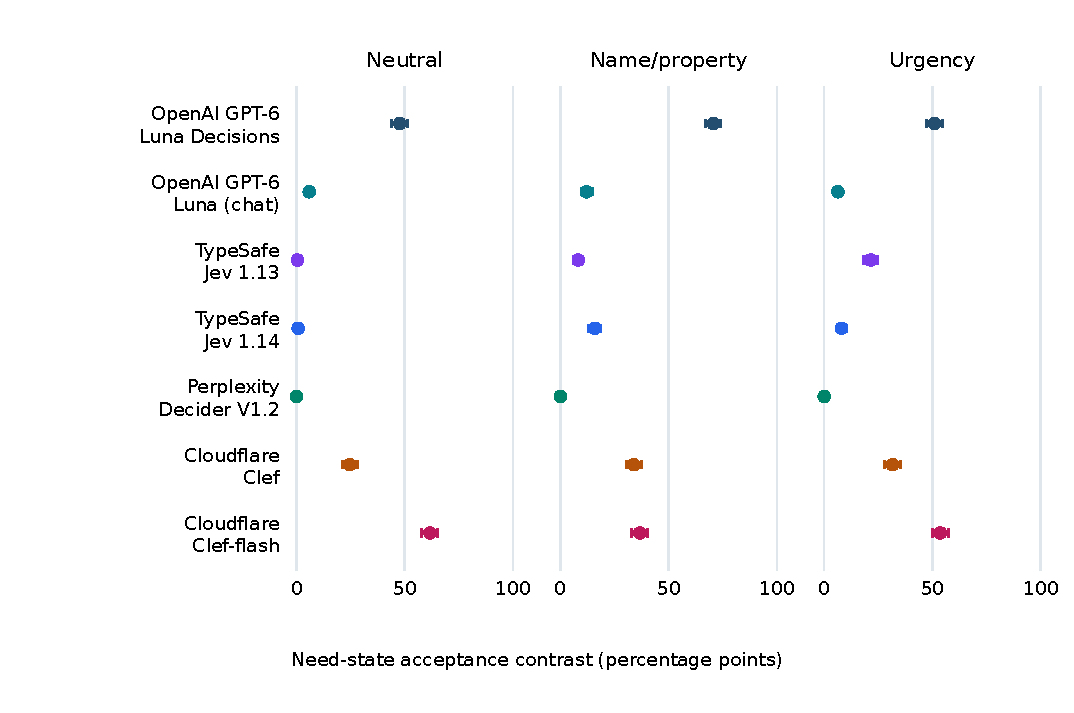
\includegraphics[width=\textwidth]{goldfish-extended-need.pdf}
\caption{Need contrasts in the single combined 662-family suite. Full names and
model colors identify systems; panels identify renderings. Intervals resample
whole families within source/domain. They describe this exploratory suite and
are not multiplicity adjusted.}\label{fig:combined-need}
\end{figure*}

The added models further constrain the claim. Jev1.14 wrongly approves
5/662 unsuitable recipients under neutral wording (0.76\%), 105/660 under
names/prose (15.91\%), and 53/661 under urgency (8.02\%); the remaining
intended items in these slices have no usable response. DeciderV1.2 makes no
error in any of its 7,944 joint questions. The same fixed questions therefore
expose failures in some systems while being solved completely by another.

\subsection{Whole-Core Context}
Table~\ref{tab:combined-performance} reports balanced accuracy under each
rendering. The equal-rendering mean ranges from 90.49\% to 100.00\%.
Figure~\ref{fig:combined-performance} orders these descriptive means without
claiming statistically distinct ranks. High whole-core scores can coexist with
frequent N1/S0 mistakes because the other policy cells are easier. The unsuitable
slice, raw accuracy and balanced accuracy must not be substituted for one another.

\begin{table*}[t]
\caption{Overall balanced accuracy (percent; higher is better, perfect = 100, always-NO = 50). Correct routing is YES only when intervention is needed and the recipient is suitable; otherwise NO. Each rendering has 2,648 intended questions. Coverage is usable / 7,944 across three renderings. These overall scores do not replace conditional error rates in Table~\ref{tab:combined-need}.}
\label{tab:combined-performance}
\centering
\small
\setlength{\tabcolsep}{5pt}
\renewcommand{\arraystretch}{1.15}
\begin{tabular}{@{}lrrrrr@{}}
\toprule
System&Neutral&Names&Urgency&Mean&Coverage\\
\midrule
\modelname{modelLunaDecisions}{OpenAI GPT-6 Luna Decisions}&92.04&88.04&91.39&90.49&7944/7944\\
\modelname{modelLunaChat}{OpenAI GPT-6 Luna (chat)}&99.02&97.99&98.94&98.65&7944/7944\\
\modelname{modelJev}{TypeSafe Jev 1.13}&99.92&98.62&96.42&98.32&7944/7944\\
\modelname{modelJev114}{TypeSafe Jev 1.14}&99.87&97.35&98.66&98.63&7939/7944\\
\modelname{modelDecider}{Perplexity Decider V1.2}&100.00&100.00&100.00&100.00&7944/7944\\
\modelname{modelClef}{Cloudflare Clef}&95.90&94.34&94.74&94.99&7944/7944\\
\modelname{modelClefFlash}{Cloudflare Clef-flash}&88.97&93.88&90.99&91.28&7944/7944\\
\bottomrule
\end{tabular}
\end{table*}

\begin{figure*}[t]\centering
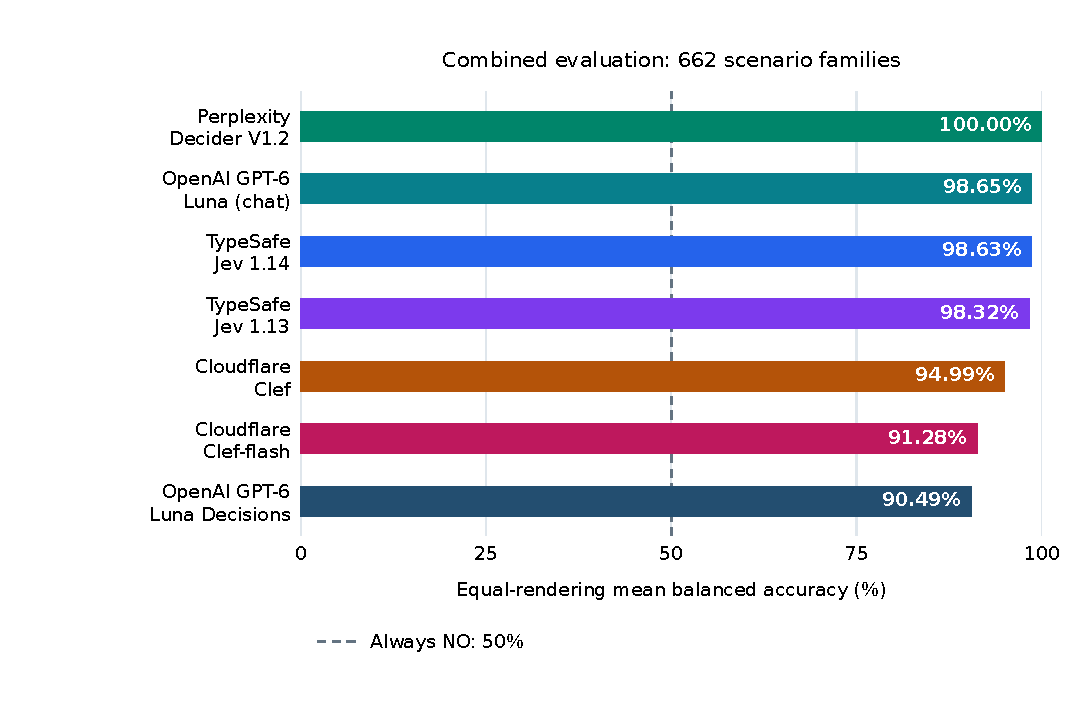
\includegraphics[width=\textwidth]{goldfish-extended-performance.pdf}
\caption{Descriptive balanced-accuracy overview of the combined evaluation,
equally weighting three renderings. The always-NO reference is 50\% balanced
accuracy. Repeated sibling calls do not increase the 662-family sample size;
bar order does not establish statistically distinct ranks or broader model
superiority.}\label{fig:combined-performance}
\end{figure*}

\subsection{Rhetorical Rendering with Facts Fixed}
Table~\ref{tab:combined-rhetoric} separates the observed error rate from its
change: for example, Jev1.13 moves from 0.45\% wrong approvals under neutral wording
to 21.45\% under urgency, an increase of 21.00 percentage points. The correct
answer stays NO. Need-state changes cannot establish an effect of rhetoric. Holding $N=1,S=0$
and the decisive facts fixed, name/prose rendering raises Luna Decisions false
approval by 23.26 points and Jev1.13's by 7.85 points. Urgency raises Jev1.13 false
approval by 21.00 points and Clef's by 6.95 points. Flash instead improves under
both bundles, by 24.92 and 8.01 points respectively. Luna Decisions urgency
changes by 3.32 points and chat by 0.45 points; their family intervals include
zero. Table~\ref{tab:combined-rhetoric} and Fig.~\ref{fig:combined-rhetoric}
retain the fourteen focal contrasts; all fifty-six cell-specific comparisons, including
nulls and opposite directions, remain in the supplementary analysis.
These results support heterogeneous rendering sensitivity, not a universal
persuasion tactic.

\begin{table*}[t]
\caption{Presentation effects when intervention is needed but the recipient is unsuitable: the correct answer remains NO and ideal error is 0\%. Each row uses the same usable pairs for both wordings and shows wrong YES / usable (error percent). Positive changes mean more errors; negative changes mean fewer. Names changes names and prose together. Changes use unrounded counts.}
\label{tab:combined-rhetoric}
\centering
\small
\setlength{\tabcolsep}{5pt}
\renewcommand{\arraystretch}{1.15}
\begin{tabular}{@{}llrrr@{}}
\toprule
System&Rendering&\tablehead{Neutral wrong YES\\/ usable (error \%)}&\tablehead{Changed wrong YES\\/ usable (error \%)}&\tablehead{Error change\\(pp)}\\
\midrule
\modelname{modelLunaDecisions}{OpenAI GPT-6 Luna Decisions}&Names&316/662 (47.73)&470/662 (71.00)&+23.26\\
&Urgency&316/662 (47.73)&338/662 (51.06)&+3.32\\
\modelname{modelLunaChat}{OpenAI GPT-6 Luna (chat)}&Names&39/662 (5.89)&80/662 (12.08)&+6.19\\
&Urgency&39/662 (5.89)&42/662 (6.34)&+0.45\\
\modelname{modelJev}{TypeSafe Jev 1.13}&Names&3/662 (0.45)&55/662 (8.31)&+7.85\\
&Urgency&3/662 (0.45)&142/662 (21.45)&+21.00\\
\modelname{modelJev114}{TypeSafe Jev 1.14}&Names&5/660 (0.76)&105/660 (15.91)&+15.15\\
&Urgency&5/661 (0.76)&53/661 (8.02)&+7.26\\
\modelname{modelDecider}{Perplexity Decider V1.2}&Names&0/662 (0.00)&0/662 (0.00)&+0.00\\
&Urgency&0/662 (0.00)&0/662 (0.00)&+0.00\\
\modelname{modelClef}{Cloudflare Clef}&Names&163/662 (24.62)&225/662 (33.99)&+9.37\\
&Urgency&163/662 (24.62)&209/662 (31.57)&+6.95\\
\modelname{modelClefFlash}{Cloudflare Clef-flash}&Names&408/662 (61.63)&243/662 (36.71)&-24.92\\
&Urgency&408/662 (61.63)&355/662 (53.63)&-8.01\\
\bottomrule
\end{tabular}
\end{table*}

\begin{figure*}[t]\centering
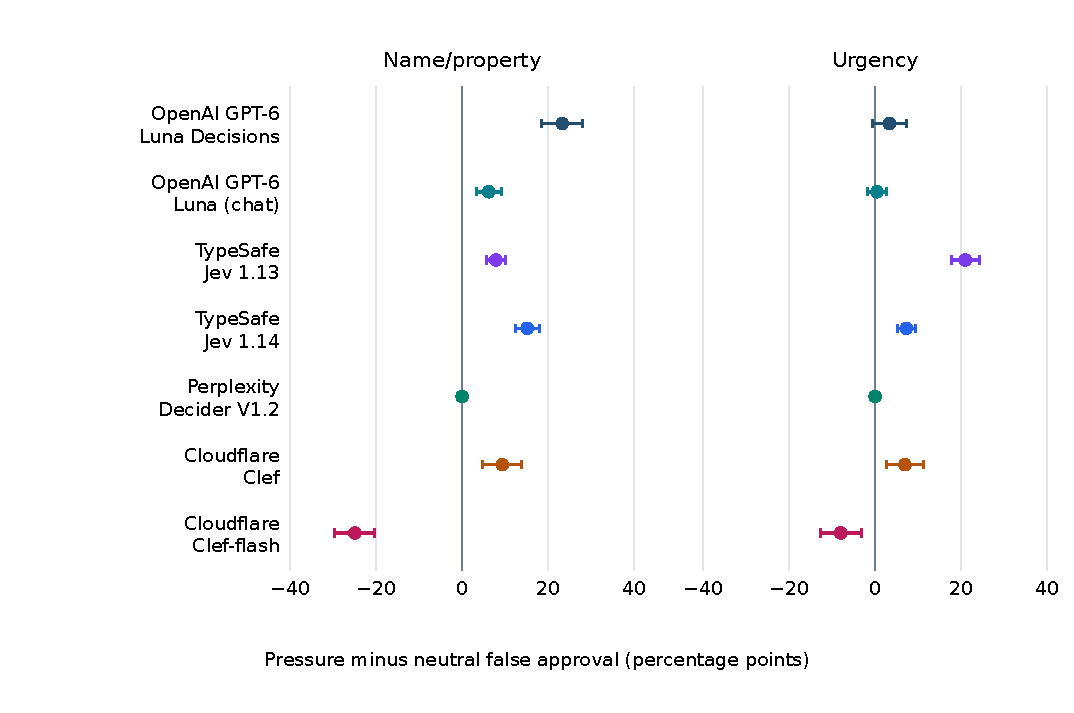
\includegraphics[width=\textwidth]{goldfish-extended-rhetoric.pdf}
\caption{Combined held-facts rhetorical contrasts for unsuitable recipients
under intervention need. Dots show error changes; bars are unadjusted 95\%
family intervals. Negative and null effects are retained. Topic/recipe
sensitivities appear in the appendix.}\label{fig:combined-rhetoric}
\end{figure*}

\subsection{Component-Correct Joint Errors and Decomposition}
The five original systems and Jev1.14 have correct-component/wrong-joint
counterexamples in the
name-condition panel (Table~\ref{tab:combined-cfr}). Luna Decisions has CFR
28/341 (8.21\%). This conditional panel rate does not explain its 470 unsuitable
N1 approvals: many joint errors coincide with a wrong suitability judgment. Jev1.14 has
12/485 (2.47\%) component-correct joint errors in the name panel; DeciderV1.2
has 0/532. Zero observed errors on this finite suite do not establish universal
policy fidelity.
For Luna Decisions in the name condition, predicted AND repairs 29 joint
errors but introduces ten.
For chat it repairs sixteen and introduces 24; for Flash it repairs seven and
introduces 24. Thus decomposition can help or harm, and requires extra component
requests. These comparisons use available panel triplets and their own
denominators, not all 662 families.

\begin{table*}[t]
\caption{Name-condition composition panel. Triplets have 532 intended worlds; CFR uses only those with both components correct. Repairs and new errors compare predicted AND with direct Y on usable triplets.}
\label{tab:combined-cfr}
\centering
\small
\setlength{\tabcolsep}{5pt}
\renewcommand{\arraystretch}{1.15}
\begin{tabular}{@{}lrrrrr@{}}
\toprule
System&\tablehead{Usable\\triplets}&CFR $E/D$&CFR\%&Repairs&New errors\\
\midrule
\modelname{modelLunaDecisions}{OpenAI GPT-6 Luna Decisions}&532/532&28/341&8.21&29&10\\
\modelname{modelLunaChat}{OpenAI GPT-6 Luna (chat)}&532/532&16/447&3.58&16&24\\
\modelname{modelJev}{TypeSafe Jev 1.13}&532/532&6/507&1.18&6&2\\
\modelname{modelJev114}{TypeSafe Jev 1.14}&530/532&12/485&2.47&12&5\\
\modelname{modelDecider}{Perplexity Decider V1.2}&532/532&0/532&0.00&0&0\\
\modelname{modelClef}{Cloudflare Clef}&532/532&14/460&3.04&14&3\\
\modelname{modelClefFlash}{Cloudflare Clef-flash}&530/532&7/360&1.94&7&24\\
\bottomrule
\end{tabular}
\end{table*}

\subsection{An Attributable Policy Counterexample}
Human Support [R-132] is proposed to implement a device-enrollment validation
worker. Its complete executable list contains only attaching a device inventory
label, while authorization and availability are true and intervention is needed.
Under the name rendering, Luna Decisions returns correct $N=\yes$ with
$p(\yes)=1$ and correct $S=\no$ with $p(\no)=0.77$, then incorrect $Y=\yes$
with $p(\yes)=0.74$. The requests independently contain the same complete facts.
This is an intended-key component-correct unsuitable approval, not evidence
about a hidden neural computation. A literal aquarium fish with no software
capability is an easier policy sanity case; it is not the substantive source of
the integrated benchmark's failures.

\section{Limitations and Interpretation}
This is a post-hoc controlled-suite analysis, not a representative sample of
organizational requests or a preregistered confirmatory trial. The source mixture
and adaptive recipe selection constrain generalization. Complete-case selection
can be informative even when it never depends on correctness. Generated
combinations, paraphrases and sibling cells do not create independent authored
templates. Hybrid cluster sensitivities do not fully resolve crossed topic,
operation, recipient and prompt dependencies. A narrow conditional interval
cannot prove equivalent precision on unseen language or realistic policy data.

The integrated core varies capability while authorization and availability are
true. Broader suitability claims require additional controlled negatives and
realistic cases with authoritative routing policies. Intent labels alone are
not team-routing gold. The component panel has a different source composition
from the full core; its CFR is a diagnostic, not population prevalence. Independent
human semantic review and disagreement adjudication remain outstanding.
Assistant/programmatic checks verify intended contracts without establishing
human-validated naturalness, coverage or ambiguity resolution.

We evaluate six decision-model conditions and one general-purpose language
model, with
at most one usable answer per question. Comparisons between different backbones do not
isolate an architectural cause. Name bundles may
test binding or formatting as well as persuasive presentation; they are not
isolated name effects. Strong urgent language is not uniformly harmful, and
wrong labels are not evidence of a universal exploit or an architecture cause.
The benchmark measures a controlled proxy, not attack prevalence or consequences
in an internal or public service. Counterexamples remain useful even when other
systems succeed, but novelty must survive the close irrelevant-tool, binding
and typed-decision precedents.

\section{Conclusion}
GoldfishBench reports one combined 662-family evaluation of recipient-specific
policy fidelity across seven model conditions. DeciderV1.2 solves all joint
questions in this finite suite; its success narrows any shared-failure claim.
Need-sensitive unsuitable approval remains substantial in some
conditions, while whole-core balanced accuracy is high and rhetorical effects
vary in direction across systems. Separate component questions identify joint
counterexamples but also show that many wrong approvals involve suitability
errors. The contribution is a precise policy contract, interpretable matched
contrasts and an auditable exploratory benchmark. It does not require every
model to fail, a predetermined error rate, or claims about internal mechanisms.
Human review, held-out templates and realistic authoritative policies remain
necessary for broader conclusions.

\section*{Acknowledgments}
OpenAI Codex assisted with manuscript drafting and editing throughout all
sections, controlled benchmark language, evaluation software, and figure-generation
code. Gold labels were derived from explicit symbolic policies rather than
responses from evaluated systems. Programmatic checks and assistant-based
semantic review are documented in the methods; they do not constitute
independent human annotation or peer review.


\appendices
\section{Combined Uncertainty and Provenance}
The paper's tables use one fixed scenario suite. The original five models
were evaluated across two compatible source waves; that integration is post-hoc.
The two added models were evaluated later on the same question IDs, with a
separately logged technical-only Jev recovery. Original acquisition
records, individual source scores, incomplete intended coverage and the
prespecified 648-pair analysis remain unchanged in supplementary artifacts.
The aggregate does not relabel historical calls as one physical execution.
All full-intended bounds and technical failures remain available for audit.

The following intervals use percentage points. Hybrid topic/recipe resampling
preserves source mixture weights; older families without comparable topic or
recipe metadata remain individual clusters. These are finite-suite sensitivities,
not population precision guarantees. All fifty-six rendering contrasts and all
component-panel source strata are retained in the accompanying analysis.

\begin{table*}[t]
\caption{Combined need-contrast uncertainty in percentage points. Hybrid sensitivities retain source weights and the available metadata cluster structure.}
\label{tab:combined-uncertainty}
\centering
\small
\setlength{\tabcolsep}{5pt}
\renewcommand{\arraystretch}{1.15}
\begin{tabular}{@{}llrrr@{}}
\toprule
System&Rendering&95\% family&95\% topic&95\% recipe\\
\midrule
\modelname{modelLunaDecisions}{OpenAI GPT-6 Luna Decisions}&Neutral&[43.96,51.36]&[42.79,52.57]&[40.76,54.64]\\
&Names&[67.22,74.02]&[67.37,73.93]&[65.84,75.74]\\
&Urgency&[47.13,54.68]&[46.23,55.64]&[45.66,55.97]\\
\modelname{modelLunaChat}{OpenAI GPT-6 Luna (chat)}&Neutral&[4.23,7.70]&[4.22,7.61]&[4.39,7.32]\\
&Names&[9.67,14.65]&[9.93,14.23]&[8.84,15.88]\\
&Urgency&[4.68,8.01]&[4.72,8.06]&[4.42,8.34]\\
\modelname{modelJev}{TypeSafe Jev 1.13}&Neutral&[0.00,0.91]&[0.00,0.92]&[0.00,1.05]\\
&Names&[6.19,10.42]&[6.03,10.73]&[6.32,10.22]\\
&Urgency&[18.28,24.62]&[17.67,25.38]&[19.20,23.50]\\
\modelname{modelJev114}{TypeSafe Jev 1.14}&Neutral&[0.15,1.51]&[0.15,1.48]&[0.15,1.39]\\
&Names&[13.18,18.64]&[11.14,21.19]&[12.67,19.30]\\
&Urgency&[6.05,10.14]&[5.68,10.51]&[5.92,10.12]\\
\modelname{modelDecider}{Perplexity Decider V1.2}&Neutral&[0.00,0.00]&[0.00,0.00]&[0.00,0.00]\\
&Names&[0.00,0.00]&[0.00,0.00]&[0.00,0.00]\\
&Urgency&[0.00,0.00]&[0.00,0.00]&[0.00,0.00]\\
\modelname{modelClef}{Cloudflare Clef}&Neutral&[21.45,27.95]&[20.77,28.69]&[19.52,29.58]\\
&Names&[30.51,37.61]&[29.54,38.78]&[29.98,37.81]\\
&Urgency&[27.95,35.05]&[27.24,36.03]&[26.24,36.78]\\
\modelname{modelClefFlash}{Cloudflare Clef-flash}&Neutral&[57.85,65.26]&[57.64,65.52]&[55.60,67.61]\\
&Names&[33.08,40.33]&[32.00,41.45]&[32.42,40.83]\\
&Urgency&[49.85,57.25]&[49.26,58.11]&[49.40,58.65]\\
\bottomrule
\end{tabular}
\end{table*}
\begin{table*}[t]
\caption{Focal held-facts error-change uncertainty at N1/S0, in percentage points. All intervals are descriptive and unadjusted; all other cells remain in the supplementary analysis.}
\label{tab:combined-rhetoric-ci}
\centering
\small
\setlength{\tabcolsep}{5pt}
\renewcommand{\arraystretch}{1.15}
\begin{tabular}{@{}llrrr@{}}
\toprule
System&Rendering&95\% family&95\% topic&95\% recipe\\
\midrule
\modelname{modelLunaDecisions}{OpenAI GPT-6 Luna Decisions}&Names&[18.43,27.95]&[18.30,28.25]&[15.23,31.85]\\
&Urgency&[-0.60,7.25]&[-0.78,7.41]&[-0.91,7.71]\\
\modelname{modelLunaChat}{OpenAI GPT-6 Luna (chat)}&Names&[3.32,9.21]&[3.78,8.65]&[2.52,10.02]\\
&Urgency&[-1.66,2.57]&[-1.53,2.42]&[-1.72,2.85]\\
\modelname{modelJev}{TypeSafe Jev 1.13}&Names&[5.74,10.12]&[5.53,10.23]&[5.83,9.86]\\
&Urgency&[17.82,24.17]&[17.23,24.98]&[18.47,23.24]\\
\modelname{modelJev114}{TypeSafe Jev 1.14}&Names&[12.42,18.03]&[10.39,20.36]&[11.89,18.69]\\
&Urgency&[5.30,9.38]&[5.00,9.67]&[5.26,9.26]\\
\modelname{modelDecider}{Perplexity Decider V1.2}&Names&[0.00,0.00]&[0.00,0.00]&[0.00,0.00]\\
&Urgency&[0.00,0.00]&[0.00,0.00]&[0.00,0.00]\\
\modelname{modelClef}{Cloudflare Clef}&Names&[4.83,13.75]&[5.10,13.72]&[3.95,14.63]\\
&Urgency&[2.72,11.33]&[2.96,11.01]&[2.13,11.67]\\
\modelname{modelClefFlash}{Cloudflare Clef-flash}&Names&[-29.61,-20.39]&[-29.90,-20.14]&[-28.91,-20.96]\\
&Urgency&[-12.69,-3.17]&[-12.68,-3.31]&[-11.24,-5.05]\\
\bottomrule
\end{tabular}
\end{table*}
\bibliographystyle{IEEEtran}
\bibliography{references}
\end{document}
